% MetricVision mid-submission report, revised version (28 Oct 2026).
% Build from report/:  latexmk -pdf mid_report_revised.tex   (or tectonic mid_report_revised.tex)
% Figures: validation/*.pdf are produced by  uv run python scripts/validate_methods.py --out report/validation
% Optional: copy the mid-report figures (kitti_00_trajectory.pdf, kitti_00_devkit.pdf, ...) into report/figures/;
% they are included in Appendix C when present.
\documentclass[11pt,a4paper]{article}
\usepackage[margin=2cm]{geometry}
\usepackage{amsmath,amssymb}
\usepackage{graphicx}
\usepackage{booktabs}
\usepackage{xcolor}
\usepackage{float}
\usepackage{enumitem}
\usepackage{microtype}
\usepackage[font=small,labelfont=bf]{caption}
\usepackage{tikz}
\usetikzlibrary{positioning,arrows.meta,fit}
\usepackage[hidelinks]{hyperref}
\setlist{nosep,leftmargin=*}
\graphicspath{{figures/}{validation/}}
\newcommand{\R}{\mathbb{R}}
\newcommand{\T}{\mathbf{T}}
\newcommand{\optfig}[2]{\IfFileExists{figures/#1}{\includegraphics[width=#2]{#1}}{}}

\title{\vspace{-1.2cm}MetricVision: Stereo Visual Odometry with a Rigid-Rig Constraint\\[2pt]\large Mid-Submission Report (revised)}
\author{Soumo Roy, Mohammed Azif, Tashmoy Ghosh}
\date{28 October 2026}

\begin{document}
\maketitle
\vspace{-0.7cm}

\begin{abstract}
\noindent We are building a stereo visual odometry (VO) pipeline from scratch that treats the calibrated two-camera rig as one rigid body. The baseline system combines a FAST/ORB stereo front end with circular KLT tracking, covariance-propagating triangulation, PnP + RANSAC, a covariance-weighted rigid-rig Levenberg--Marquardt (LM) refinement and fused landmark anchors. It tracks every frame of KITTI~00 and EuRoC~MH\_01 and reaches a KITTI devkit drift of 1.39\% and 0.50$^\circ$/100\,m, against 1.73\% and 0.79$^\circ$/100\,m for a dense SGBM baseline with the same back end. A review against our research questions then exposed four weaknesses: an inconsistent noise model, a RANSAC that ignores the right image, over-confident fused anchors and KLT drift. We have implemented and tested fixes for each, together with rig baselines and a rig-consistency monitor. Controlled experiments confirm the mechanisms. The pose NEES is 5.9 (ideal 6), against 1.5 before the fix. The anchor NEES is 3.3 (ideal 3), where it otherwise grows to 12. Inverse depth removes an 8\% fused-depth bias at 100\,m. Re-alignment keeps track error near 0.04\,px, where chained KLT drifts to 2\,px. A first RQ3 experiment shows that a 0.1$^\circ$ yaw error of the right camera causes about 7\% per-frame translation error, yet is invisible to the vertical-disparity check, which sets our research direction.
\end{abstract}

\section{Introduction and problem statement}\label{sec:problem}
A monocular camera cannot observe metric scale. A calibrated stereo rig recovers depth in metres from its known baseline in every frame, which makes stereo VO the natural ego-motion sensor for robots without GPS. Most stereo pipelines still treat the two images loosely: as a depth source for one camera, or as two independently tracked views. We instead impose the physical fact that the two cameras are bolted together: one pose per stereo frame explains the observations in both images through the fixed calibrated extrinsic.

\paragraph{Formal statement.}
Let $\{(I^L_k, I^R_k)\}_{k=0}^{N}$ be a synchronised stereo sequence from a rig with known intrinsics and fixed extrinsic $\T_{RL}\in SE(3)$. After rectification both cameras share $\mathbf K = (f_x, f_y, c_x, c_y)$, and $\T_{RL}$ reduces to a translation by the baseline $\mathbf b = (B, 0, 0)^\top$. We seek the left-camera poses $\T_{W,k}$ ($\T_{W,0} = \mathbf I$). The estimate must be \emph{causal}, \emph{metric} (evaluated without scale correction), \emph{rigid-rig consistent} (a single unknown pose per frame, so a landmark $\mathbf P_j$ projects as $\pi(\mathbf K, \T_{k,W}\mathbf P_j)$ into the left image and as $\pi(\mathbf K, \T_{k,W}\mathbf P_j - \mathbf b)$ into the right) and \emph{real-time} on a laptop CPU. Given landmarks $\mathbf P_j$ with covariances $\Sigma_j$, each frame solves
\begin{equation}
  \T_{k,W}^\ast = \arg\min_{\T\in SE(3)} \sum_{j\in\mathcal I_k} \rho_H\!\big(\mathbf r_j(\T)^\top \Sigma_{r,j}^{-1}\, \mathbf r_j(\T)\big),
  \quad
  \mathbf r_j(\T) = \begin{bmatrix} \mathbf u^L_{kj} - \pi(\mathbf K, \T\mathbf P_j) \\ u^R_{kj} - \pi_u(\mathbf K, \T\mathbf P_j - \mathbf b)\end{bmatrix}\!\in\R^3,
  \label{eq:problem}
\end{equation}
where $\mathcal I_k$ is the set of inlier tracks, $\rho_H$ is the Huber loss and $\Sigma_{r,j}$ is the residual covariance induced by $\Sigma_j$ and the pixel noise $\sigma$. Success means low drift (ATE, RPE, KITTI devkit~\cite{kitti,sturm,zhang_eval}) with no tracking loss. Loop closure, IMU fusion and dynamic scenes are out of scope.

\paragraph{Research questions.} \textbf{RQ1} (coupling): how much drift does the rigid-rig coupling~\eqref{eq:problem} remove, compared with left-only, independent per-camera and loosely averaged estimation? \textbf{RQ2} (uncertainty): does covariance weighting beat the usual depth-gating heuristic, and are the resulting estimates statistically consistent? \textbf{RQ3} (fragility): how sensitive is the rigid constraint to extrinsic error, and can such error be detected online? RQ3 is our intended publication direction.

\section{Literature review}\label{sec:lit}
\paragraph{Feature-based stereo VO.} Nist\'er et al.~\cite{nister} introduced real-time VO, and the tutorial of Scaramuzza and Fraundorfer~\cite{vo_tutorial1,vo_tutorial2} establishes 3D-to-2D (PnP) estimation as more accurate than 3D-to-3D alignment. Libviso~\cite{kitt} and StereoScan/libviso2~\cite{stereoscan} contribute grid bucketing, \emph{circular matching} and RANSAC that scores each hypothesis on \emph{both} images of the rig, which our stereo RANSAC adopts. SOFT~\cite{soft} shows that long-lived, carefully selected tracks make frame-to-frame stereo VO competitive. Badino et al.~\cite{badino} integrate each feature over its track history, which motivates our fused anchors. S-PTAM~\cite{sptam} and ORB-SLAM2/3~\cite{orbslam2,orbslam3} add keyframes, bundle adjustment and loop closure. ORB-SLAM2 uses the same 3-D stereo residual $(u_L, v_L, u_R)$ as~\eqref{eq:problem}.

\paragraph{Direct methods.} SVO~\cite{svo}, DSO~\cite{dso} and Stereo DSO~\cite{stereodso} minimise photometric error. SVO's alignment of features against a fixed reference patch inspires our drift correction (Sec.~\ref{sec:realign}).

\paragraph{Rigid multi-camera constraints and calibration.} Pless~\cite{pless} models a rigid camera set as one generalised camera, and Kneip et al.~\cite{npnp} solve its absolute pose. Coupling views to one rig pose removes redundant degrees of freedom, which is the hypothesis behind RQ1. The constraint is only as good as the calibration. Cvi\v{s}i\'c et al.~\cite{recalib} recalibrated the KITTI cameras and reduced the drift of SOFT2, ORB-SLAM2 and VISO2 by 25--30\% (VISO2: 1.62$\to$1.11\%). Calibration error is therefore a leading error source in stereo VO, which motivates RQ3.

\paragraph{Estimation and uncertainty.} RANSAC~\cite{ransac} with minimal P3P solvers~\cite{p3p,ap3p} and MSAC scoring~\cite{msac} provides robust initial poses. LM~\cite{levenberg,marquardt} on $SE(3)$ uses left-perturbation increments~\cite{barfoot,sola} as in bundle adjustment~\cite{triggs}. Matthies and Shafer~\cite{matthies} showed that stereo triangulation error grows with $Z^2$ along the ray and that covariance weighting improves motion estimates. Civera et al.~\cite{inverse_depth} showed that inverse depth is close to Gaussian where depth is not, which motivates our inverse-depth anchors. Benchmarks are KITTI~\cite{kitti} ($B = 0.54$\,m) and EuRoC~\cite{euroc} ($B = 0.11$\,m), evaluated with evo~\cite{evo} after Umeyama alignment~\cite{umeyama}.

\section{Method and progress}\label{sec:method}
The code is written in Python (OpenCV, NumPy) as a modular, registry-based package. It has 33 unit and end-to-end tests (19 at the first version of this report). Every upgrade below is a configuration switch (\texttt{--set section.key=value}), so each one can be ablated in isolation. Fig.~\ref{fig:pipeline} shows the per-frame loop and Table~\ref{tab:progress} compares progress with the proposal.

\begin{figure}[t]
\centering
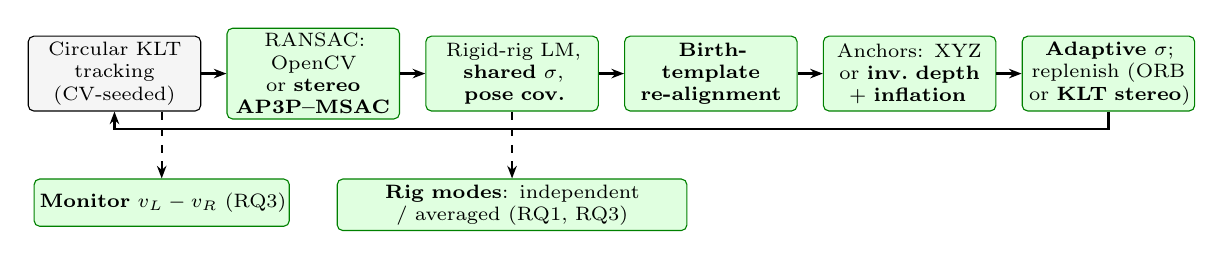
\begin{tikzpicture}[node distance=0.32cm and 0.32cm, every node/.style={font=\scriptsize, align=center},
  box/.style={draw, rounded corners=2pt, minimum height=0.95cm, inner sep=2pt, text width=2.05cm},
  new/.style={box, fill=green!12, draw=green!50!black}, old/.style={box, fill=gray!8},
  arr/.style={-{Stealth[length=1.6mm]}, thick}]
\node[old] (track) {Circular KLT\\tracking (CV-seeded)};
\node[new, right=of track] (ransac) {RANSAC: OpenCV or \textbf{stereo AP3P--MSAC}};
\node[new, right=of ransac] (lm) {Rigid-rig LM, \textbf{shared $\sigma$}, \textbf{pose cov.}};
\node[new, right=of lm] (realign) {\textbf{Birth-template re-alignment}};
\node[new, right=of realign] (anchor) {Anchors: XYZ or \textbf{inv.\ depth} + \textbf{inflation}};
\node[new, right=of anchor] (noise) {\textbf{Adaptive $\sigma$}; replenish (ORB or \textbf{KLT stereo})};
\draw[arr] (track) -- (ransac); \draw[arr] (ransac) -- (lm); \draw[arr] (lm) -- (realign);
\draw[arr] (realign) -- (anchor); \draw[arr] (anchor) -- (noise);
\draw[arr] (noise.south) -- ++(0,-0.22) -| (track.south);
\node[new, below=0.85cm of lm, text width=4.3cm, minimum height=0.6cm] (rig) {\textbf{Rig modes}: independent / averaged (RQ1, RQ3)};
\node[new, below=0.85cm of track, text width=3.1cm, minimum height=0.6cm, xshift=0.6cm] (mon) {\textbf{Monitor} $v_L - v_R$ (RQ3)};
\draw[arr, dashed] (lm.south) -- (rig.north); \draw[arr, dashed] ([xshift=0.6cm]track.south) -- (mon.north);
\end{tikzpicture}
\vspace{-0.15cm}
\caption{Per-frame loop of the sparse pipeline. Grey: mid-report components; green bold: additions since the first version (all switchable).}\label{fig:pipeline}
\vspace{-0.35cm}
\end{figure}

\begin{table}[t]
\centering\small
\caption{Progress against the proposed timeline.}\label{tab:progress}
\vspace{-0.2cm}
\begin{tabular}{p{1.6cm}p{5.0cm}p{9.0cm}}
\toprule
Week & Planned & Status \\
\midrule
2 (Oct 12--18) & Stereo matching, triangulation with covariance, circular KLT & \textbf{Done} (Sec.~\ref{sec:frontend}). \\
3 (Oct 19--24) & PnP + RANSAC; first ATE/RPE on KITTI~00, EuRoC MH\_01 & \textbf{Done.} Full sequences with zero failures; KITTI devkit metric ported (Sec.~\ref{sec:results}). \\
4 (Oct 25--31) & Rigid-rig LM with analytic Jacobians & \textbf{Done}, Jacobians verified numerically. \textbf{Also done early:} covariance weighting (planned for week~5), fused anchors, and the method upgrades of Secs.~\ref{sec:ransac}--\ref{sec:rig} with tests and controlled validation (Sec.~\ref{sec:validation}). \\
\bottomrule
\end{tabular}
\vspace{-0.4cm}
\end{table}

\subsection{Stereo front end}\label{sec:frontend}
FAST corners are bucketed on a $12{\times}4$ grid (quota $N_{\max}/48$, $N_{\max} = 1500$), with discs around existing tracks masked out. Stereo association uses either of two matchers. The first is the mid-report's ORB matcher: brute-force Hamming with an epipolar mask ($|v_R - v_L| \le 1.5$\,px, $d\in[1, 160]$\,px), a ratio test and a mutual check, followed by single-level KLT refinement of $u_R$. The second, \textbf{new}, is direct sub-pixel KLT from left to right, seeded with the median disparity of existing tracks and accepted only if a right-to-left back-check closes within 0.5\,px. It can be combined with Shi--Tomasi minimum-eigenvalue ranking~\cite{shi_tomasi}, which favours well-conditioned KLT windows, and with a low-threshold FAST pass that fills only empty cells (for low-texture scenes). Triangulation $Z = f_xB/d$ propagates independent noise $\sigma$ on $(u_L, v_L, u_R)$ to $\Sigma_P = \sigma^2 JJ^\top$, so $\sigma_Z = \sqrt2\,\sigma Z^2/(f_xB)$. A circular KLT check ($L_k\!\to\!L_{k+1}\!\to\!R_{k+1}\!\to\!R_k$, 1\,px), seeded by projecting landmarks with a constant-velocity prediction, keeps tracks over time.

\subsection{Robust initial pose: stereo RANSAC}\label{sec:ransac}
The mid-report used \texttt{cv2.solvePnPRansac} (iterative solver, 2\,px threshold, 200 iterations), which judges inliers on the \emph{left} image only. A wrong stereo match whose error lies only in $u_R$ therefore enters the LM. The \textbf{stereo RANSAC} draws minimal AP3P~\cite{ap3p} hypotheses and scores each with MSAC~\cite{msac} on $e_j = \max(|\Delta u_L|, |\Delta v_L|, |\Delta u_R|)$, with $u_R = u_L - f_xB/z$. This enforces the rig model inside RANSAC, as libviso2 does~\cite{stereoscan}. The constant-velocity prior is scored first as a free hypothesis. The number of iterations adapts to the inlier ratio ($1 - w^3$ rule, confidence 0.999), and the sampler is seeded for reproducibility. Fewer than 15 inliers counts as a tracking failure: the pose coasts on the motion model and the front end re-initialises.

\subsection{Rigid-rig LM with a shared, calibrated noise model}\label{sec:lm}
The LM minimises~\eqref{eq:problem} with the update $\T\leftarrow\exp(\boldsymbol\delta^\wedge)\T$, $\boldsymbol\delta = (\boldsymbol\rho,\boldsymbol\phi)$, and analytic Jacobians $\partial\mathbf p/\partial\boldsymbol\delta = [\mathbf I \mid -[\mathbf p]_\times]$ and $\partial\pi/\partial\mathbf p$. Residuals are whitened by $\Sigma_{r,j} = \tfrac{\partial\mathbf r}{\partial\mathbf P}\Sigma_j\tfrac{\partial\mathbf r}{\partial\mathbf P}^{\!\top} + \sigma^2\mathbf I$, so far points are down-weighted smoothly rather than cut off. The Huber threshold is $2\sigma$ (applied via IRLS), and points with $\|\mathbf e\|^2 > \chi^2_3(0.99) = 11.34$ are dropped after convergence. The 3-D residual omits $v_R$: in a rectified rig it carries no depth information, and on EuRoC it imported rectification error (per-frame rotation error 0.014$^\circ$ vs.\ 0.010$^\circ$ without it).

\textbf{Change: one noise model.} The mid-report LM assumed $\sigma = 1$\,px while triangulation assumed 0.5\,px, so whitened residuals, the $\chi^2$ gate and the implied uncertainty were mis-scaled. The LM now uses the same $\sigma$ as triangulation. \textbf{Addition: pose covariance.} The LM now returns $\Sigma_{\boldsymbol\delta} = (\sum_j w_j \mathbf J_j^\top\mathbf J_j)^{-1}$ over the whitened, IRLS-weighted inlier Jacobians, together with the per-point whitened residuals $e_j^2$. These enable consistency (NEES) analysis for RQ2 and drive Secs.~\ref{sec:anchor}--\ref{sec:noise}.

\subsection{Landmark anchors: inverse depth and pose-uncertainty inflation}\label{sec:anchor}
Re-triangulating each track every frame chains the triangulation error into the trajectory. On KITTI~00 this produced a yaw bias of $-33^\circ$ over the sequence. Each track therefore keeps an \emph{anchor} from its birth frame and fuses every re-observation $(\mathbf P', \Sigma')$ in information form, $\Sigma_j \leftarrow (\Sigma_j^{-1} + \Sigma'^{-1})^{-1}$, $\mathbf P_j \leftarrow \Sigma_j(\Sigma_j^{-1}\mathbf P_j + \Sigma'^{-1}\mathbf P')$~\cite{badino}. Two weaknesses remain, and each now has a switchable fix.
(i)~\emph{XYZ is a poor Gaussian model for distant points}: depth is a nonlinear function of disparity, so XYZ fusion is biased (Sec.~\ref{sec:validation}). \textbf{Inverse-depth anchors} store $\rho = 1/Z$ on the ray of the birth pixel. Re-observations are mapped into the birth camera and fused by a 1-D Kalman update ($\mathrm{var}\,\rho = \mathrm{var}\,Z/Z^4$), behind a $\chi^2_1$ gate of 9 that rejects inconsistent observations. The world point and its covariance are reconstructed from $(u, v, \rho)$ and the birth pose.
(ii)~\emph{Fusion treats each re-observation as independent}, but every observation inherits the error of the pose that produced it, so the anchor covariance shrinks without bound. \textbf{Pose inflation} adds $\mathbf J\Sigma_{\boldsymbol\delta}\mathbf J^\top$, with $\mathbf J = -\mathbf R_{WC}[\mathbf I \mid -[\mathbf X_C]_\times]$, to each new observation using the LM covariance. Distant points are inflated more because of the lever arm.

\subsection{Drift correction by birth-template re-alignment}\label{sec:realign}
Chained translation-only KLT accumulates a small error at every step from unmodelled patch rotation and scale. Anchored landmarks, however, are matched to the \emph{current} pixel, so this drift becomes a systematic landmark--observation mismatch. Every $N$ frames ($N = 5$), each track at least 3 frames old is re-aligned against a fixed template from its birth image, following SVO's feature alignment~\cite{svo}. The local affine warp $\partial\mathbf u_k/\partial\mathbf u_{\mathrm{birth}}$ is predicted from both poses and the anchor depth (fronto-parallel patch). Gauss--Newton then estimates a 2-D translation plus gain and bias for all tracks at once, and $u_R$ is re-matched by KLT. Corrections above 2\,px, degenerate warps and epipolar violations end the track.

\subsection{Adaptive noise}\label{sec:noise}
If the noise model is right, the whitened residuals of the inliers follow $\chi^2_3$. The pipeline therefore re-estimates $\sigma \leftarrow \sigma\sqrt{\mathrm{med}(e_j^2)/\mathrm{med}(\chi^2_3)}$, smoothed by an exponential moving average (rate 0.05) and clamped to $[0.1, 3]$\,px. The same $\sigma$ drives triangulation, weighting and gating on every dataset, including our RealSense D455.

\subsection{Rig models and rig-consistency monitoring}\label{sec:rig}
For RQ1 and RQ3 the back end can also run in two weaker modes. In \emph{independent} mode, left and right poses are estimated separately (12~DoF, mono PnP + LM on the same anchors), and the implied extrinsic $\T_R\T_L^{-1}$ is compared with calibration and logged. In \emph{averaged} mode, the two estimates are combined by an $SE(3)$ average (chordal-mean rotation, mean translation). Every frame also logs the median and MAD of $v_L - v_R$ over all tracked pairs, the predicted pose $\sigma$ and the noise estimate. A depth gate (ignore points beyond $40B$) serves as the heuristic baseline that covariance weighting must beat (RQ2), and KITTI can be run with a replacement calibration file~\cite{recalib} or a scaled baseline.

\section{Results}\label{sec:results}
\subsection{Full-sequence benchmark (baseline system)}
\textbf{Setup.} We evaluate on KITTI~00 (4541 frames, 3.7\,km) and EuRoC MH\_01 (3682 frames, camera poses mapped to the body frame). ATE is the RMSE after $SE(3)$ alignment without scale, RPE is frame-to-frame, and $t_\mathrm{rel}$, $r_\mathrm{rel}$ are KITTI devkit averages over 100--800\,m. Each configuration is one deterministic run on a 16-core laptop CPU with two runs in parallel. Timing differences below ${\sim}15$\,ms are therefore noise. All 18 runs track every frame. These runs predate the upgrades and use the mid-report setting (LM $\sigma = 1$\,px), which the code reproduces exactly.

\begin{table}[t]
\centering\scriptsize\setlength{\tabcolsep}{3.5pt}
\caption{Full-sequence results of the baseline system. ``f2f'': landmarks re-triangulated every frame; ``birth''/``fused'': per-track anchors. Dense rows use our LM with left residuals only. Bold: best per column.}\label{tab:results}
\vspace{-0.2cm}
\begin{tabular}{lrrrrr@{\hskip 10pt}rrr}
\toprule
& \multicolumn{5}{c}{KITTI 00 (4541 frames, 3.7 km)} & \multicolumn{3}{c}{EuRoC MH\_01 (3682 frames)} \\
\cmidrule(lr){2-6}\cmidrule(lr){7-9}
Method & ATE [m] & $t_\mathrm{rel}$ [\%] & $r_\mathrm{rel}$ [$^\circ$/100m] & RPE$_t$ [cm] & ms & ATE [cm] & RPE$_t$ [mm] & ms \\
\midrule
Dense ORB+SGBM, OpenCV-LM & 10.95 & 1.87 & 0.88 & 5.12 & 44 & 9.5 & 9.1 & 31 \\
Dense ORB+SGBM, our LM & \textbf{8.97} & 1.73 & 0.79 & 4.93 & 49 & 13.7 & 8.9 & 36 \\
Dense SIFT+SGBM, our LM & 10.36 & 1.41 & 0.52 & 2.93 & 83 & \textbf{4.9} & 3.1 & 67 \\
Sparse f2f, PnP only & 29.73 & 2.65 & 1.06 & \textbf{2.63} & 71 & 7.8 & \textbf{1.1} & 30 \\
Sparse f2f, OpenCV-LM & 30.04 & 2.68 & 1.07 & \textbf{2.63} & 52 & 7.4 & \textbf{1.1} & 30 \\
Sparse f2f, rig-LM & 23.70 & 2.30 & 0.90 & \textbf{2.63} & 57 & 8.4 & \textbf{1.1} & 29 \\
Sparse birth anchors, rig-LM & 11.20 & 1.45 & 0.51 & 2.75 & 60 & 8.0 & 1.5 & 32 \\
Sparse fused anchors, OpenCV-LM & 11.50 & 1.44 & 0.52 & 2.69 & 52 & 10.8 & 1.3 & 24 \\
Sparse fused anchors, rig-LM (proposed) & 10.38 & \textbf{1.39} & \textbf{0.50} & 2.67 & 66 & 5.2 & \textbf{1.1} & 30 \\
\bottomrule
\end{tabular}
\vspace{-0.35cm}
\end{table}

\textbf{Anchoring is the largest effect.} With the same front end and rig LM, KITTI ATE falls from 23.7\,m (f2f) to 11.2\,m (birth) and 10.4\,m (fused), and $t_\mathrm{rel}$ from 2.30\% to 1.39\%. The proposed configuration has the lowest devkit drift of all variants. Dense ORB has the lowest KITTI ATE, but ATE depends heavily on where along the loop the drift occurs, so the devkit metric is our primary KITTI measure. \textbf{Rigid-rig LM.} On the same inliers, our LM lowers KITTI ATE relative to OpenCV's monocular LM in every pairing (dense $10.95\!\to\!8.97$\,m, f2f $30.0\!\to\!23.7$\,m, fused $11.5\!\to\!10.4$\,m). On EuRoC the effect is mixed, and more sequences are needed. \textbf{Cost.} The sparse pipeline runs at 14--19\,FPS on KITTI and 31--42\,FPS on EuRoC. Its frame-to-frame translation error is $2\times$ lower than dense ORB on KITTI and $8\times$ lower on EuRoC. Stereo re-detection dominates runtime because it runs on almost every frame (about 550 surviving tracks against a 1050-track threshold).

\textbf{What these runs cannot answer.} The comparison ``rig-LM vs.\ OpenCV-LM'' changes the right-image residual, covariance weighting, the Huber kernel and $\sigma$ \emph{at once}, so it does not isolate the effect of the rigid constraint (RQ1) or of weighting (RQ2). The ablation of Sec.~\ref{sec:plan} changes one factor at a time.

\subsection{Controlled validation of the upgrades}\label{sec:validation}
Each mechanism was tested with ground truth in Monte Carlo experiments that use the KITTI camera ($f_x = 718.9$\,px, $B = 0.537$\,m, $\sigma = 0.5$\,px). They are reproducible with \texttt{scripts/validate\_methods.py}. Table~\ref{tab:validation} and Fig.~\ref{fig:validation} summarise the results.

\begin{table}[t]
\centering\scriptsize\setlength{\tabcolsep}{4pt}
\caption{Controlled validation (KITTI camera, $\sigma = 0.5$\,px; ideal values in brackets).}\label{tab:validation}
\vspace{-0.2cm}
\begin{tabular}{p{3.3cm}p{6.0cm}p{6.6cm}}
\toprule
Mechanism & Experiment & Result \\
\midrule
Shared noise model (\ref{sec:lm}) & 300 frame pairs, 300 points at 5--80\,m, $\sim$0.9\,m motion; mean pose NEES & LM $\sigma = 0.5$\,px: \textbf{5.85} [6]; mid-report LM $\sigma = 1$\,px: 1.48 (covariance $4\times$ too pessimistic, $\chi^2$ gate never fires) \\
Stereo RANSAC (\ref{sec:ransac}) & 100 trials, 20\% gross left outliers + 10\% right-only outliers & Right-only outliers accepted: OpenCV 97\%, stereo \textbf{0\%}. Final error after the LM is equal (0.22\,cm, 0.005$^\circ$) because the LM $\chi^2$ test catches them too; RANSAC time 3--5\,ms vs.\ 1.9\,ms (Python) \\
Inverse-depth anchors (\ref{sec:anchor}) & Depth bias after fusing 20 observations of one point & 30\,m: XYZ $-0.8\%$, $\rho$ $+0.02\%$; 60\,m: $-3.2\%$ vs.\ $+0.07\%$; 100\,m (3.9\,px disparity): \textbf{$-8.0\%$ vs.\ $+0.16\%$} \\
Pose inflation (\ref{sec:anchor}) & 25\,m point fused over 30 frames whose poses carry 1\,cm / 0.05$^\circ$ error; anchor NEES & No inflation: grows to \textbf{12.2}; with inflation: \textbf{3.25} [3] \\
Re-alignment (\ref{sec:realign}) & Textured plane at 20\,m, 0.25\,m forward per frame ($2\times$ zoom over 40 frames), 98 tracks & Median track error, chained KLT: 0.26 / 0.65 / 2.02\,px after 10 / 20 / 40 frames; re-aligned: \textbf{0.02 / 0.04\,px} after 20 / 40 frames \\
KLT stereo matching (\ref{sec:frontend}) & Synthetic plane, analytic disparity 13.5\,px & Median disparity error $< 0.1$\,px, 90th percentile $< 0.3$\,px \\
\bottomrule
\end{tabular}
\vspace{-0.3cm}
\end{table}

\begin{figure}[t]
\centering
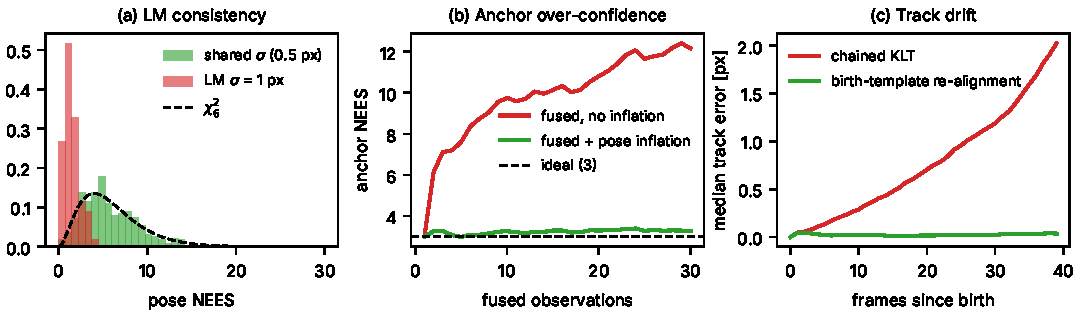
\includegraphics[width=\linewidth]{validation.pdf}
\vspace{-0.6cm}
\caption{(a) Pose NEES of the rig LM against $\chi^2_6$: the shared noise model is consistent, while the mid-report setting is not. (b) Anchor NEES during fusion with unmodelled pose error: without inflation the anchor becomes over-confident. (c) Track error against ground truth: chained KLT drifts, birth-template re-alignment does not.}\label{fig:validation}
\vspace{-0.35cm}
\end{figure}

\textbf{End-to-end check.} On a synthetic stereo sequence every option, alone and combined, tracks all frames with ATE 0.12--0.60\,mm (Appendix~\ref{app:synthetic}). This shows that the integration works, not which method is best.

\subsection{First RQ3 experiment: sensitivity to extrinsic rotation error}\label{sec:rq3}
In this experiment the right camera is rotated away from its calibration while the pipeline keeps assuming the nominal rig. Landmarks are triangulated with the wrong rig in one frame, and the next pose is estimated either with the rigid-rig LM or with the left-only LM (60 trials per level, Fig.~\ref{fig:extrinsic}). Three findings follow:
\begin{enumerate}
  \item A \textbf{yaw} (toe-in) error biases every disparity by $f_x\tan\theta$ (1.25\,px at 0.1$^\circ$). Translation error per frame reaches 6.9\% at 0.1$^\circ$ and 30\% at 0.5$^\circ$, \emph{for the rigid and left-only estimators alike}, because both use the miscalibrated triangulation. The rigid LM keeps rotation error 2--3$\times$ lower (0.012$^\circ$ vs.\ 0.033$^\circ$ at 0.1$^\circ$).
  \item A \textbf{pitch} error produces a large vertical disparity (1.3\,px at 0.1$^\circ$) but barely affects the pose, because the 3-D residual ignores $v_R$. A \textbf{roll} error produces no median offset, but the MAD grows (0.9\,px at 0.1$^\circ$, 3.8\,px at 0.5$^\circ$), and it degrades translation only mildly.
  \item The most damaging error, yaw, is therefore \emph{invisible} to the vertical-disparity check. Detecting it needs a disparity-scale consistency signal instead, for example agreement between stereo depth and the depth implied by temporal motion. This is the core of our planned ``detect-then-free'' extrinsic estimator.
\end{enumerate}
These observations agree with the large KITTI recalibration gains reported in~\cite{recalib}.

\begin{figure}[t]
\centering
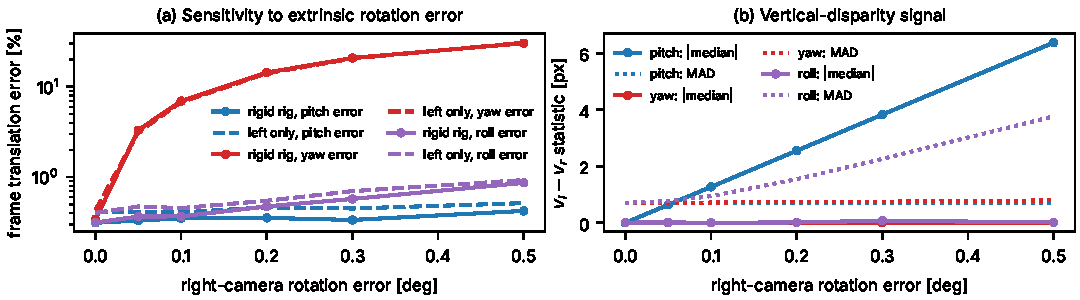
\includegraphics[width=\linewidth]{extrinsic.pdf}
\vspace{-0.6cm}
\caption{RQ3 preview. (a) Per-frame translation error (log scale) against the rotation error of the right camera, for the rigid-rig and left-only LM. (b) The logged vertical-disparity statistics: pitch shifts the median, roll widens the spread, and yaw leaves both unchanged.}\label{fig:extrinsic}
\vspace{-0.35cm}
\end{figure}

\section{Ablation protocol and timeline}\label{sec:plan}
\textbf{One-factor ablation (scripted, \texttt{scripts/run\_ablations.sh}).} The reference is the proposed configuration with the shared noise model. Each run changes one factor:
\begin{itemize}
  \item RQ1: left-only LM; independent and averaged rig modes.
  \item RQ2: no covariance weighting; no weighting but a $40B$ depth gate; no Huber; $\sigma = 1$\,px.
  \item Method upgrades, one at a time: stereo RANSAC, inverse depth, inflation, adaptive $\sigma$, re-alignment, KLT stereo matching. Then all of them together.
  \item RQ3: the full configuration on recalibrated KITTI~\cite{recalib}.
\end{itemize}
The protocol covers KITTI~00--10 and the EuRoC sequences. Statistics will use paired per-segment Wilcoxon tests and bootstrap confidence intervals. We keep an upgrade only if it improves drift or consistency (ANEES) on real data. The synthetic results above do not show that it does.

\begin{table}[H]
\centering\footnotesize
\vspace{-0.2cm}
\begin{tabular}{p{2.1cm}p{10.5cm}p{3.0cm}}
\toprule
Week & Tasks & Deliverable \\
\midrule
5 (Nov 1--7) & Ablation runs on KITTI 00/05/07 and EuRoC MH\_01; fix the final configuration. Sliding-window bundle adjustment (5--7 keyframes, 3-D stereo residual, Schur complement, oldest keyframe fixed). Wheelchair D455 recording (ChArUco calibration, 5 sequences) & Ablation table; full pipeline \\
6 (Nov 8--14) & KITTI 00--10, EuRoC (11 sequences) and wheelchair (FTE). Libviso2 and ORB-SLAM3 (VO mode) baselines. KITTI default vs.\ recalibrated. Consistency (ANEES) study & ATE / RPE / FTE / ANEES tables \\
7 (Nov 15--21) & Per-stage latency on laptop and Jetson (ROS~2 node); RQ3 extrinsic perturbation study; report writing & Draft final report \\
8 (Nov 22--23) & Final submission (Nov 23): code and reproduction scripts & Final report + code \\
-- (Nov 26) & Demo: live wheelchair run and replay of recorded sequences & Demo \\
\bottomrule
\end{tabular}
\vspace{-0.2cm}
\end{table}
\noindent\textbf{Risks.} Python bundle adjustment may be slow, so we use a Schur complement and a small window. Re-alignment costs about 120\,ms per call, so it runs only every 5 frames. Some upgrades may not help on real data; the ablation decides, and the baseline already meets the course requirements.

\begingroup\small
\begin{thebibliography}{99}\setlength{\itemsep}{0pt}
\bibitem{nister} D.~Nist\'er, O.~Naroditsky, J.~Bergen, ``Visual odometry,'' CVPR, 2004.
\bibitem{vo_tutorial1} D.~Scaramuzza, F.~Fraundorfer, ``Visual odometry [Tutorial] Part I,'' IEEE Robot. Autom. Mag., 18(4), 2011.
\bibitem{vo_tutorial2} F.~Fraundorfer, D.~Scaramuzza, ``Visual odometry: Part II,'' IEEE Robot. Autom. Mag., 19(2), 2012.
\bibitem{kitt} B.~Kitt, A.~Geiger, H.~Lategahn, ``Visual odometry based on stereo image sequences with RANSAC-based outlier rejection scheme,'' IEEE IV, 2010.
\bibitem{stereoscan} A.~Geiger, J.~Ziegler, C.~Stiller, ``StereoScan: Dense 3D reconstruction in real-time,'' IEEE IV, 2011.
\bibitem{soft} I.~Cvi\v{s}i\'c, I.~Petrovi\'c, ``Stereo odometry based on careful feature selection and tracking,'' ECMR, 2015.
\bibitem{recalib} I.~Cvi\v{s}i\'c, I.~Markovi\'c, I.~Petrovi\'c, ``Recalibrating the KITTI dataset camera setup for improved odometry accuracy,'' ECMR, 2021.
\bibitem{badino} H.~Badino, A.~Yamamoto, T.~Kanade, ``Visual odometry by multi-frame feature integration,'' ICCV Workshops, 2013.
\bibitem{sptam} T.~Pire, T.~Fischer, G.~Castro, P.~De~Crist\'oforis, J.~Civera, J.~Jacobo~Berlles, ``S-PTAM: Stereo parallel tracking and mapping,'' Robot. Auton. Syst., 93, 2017.
\bibitem{orbslam2} R.~Mur-Artal, J.~D.~Tard\'os, ``ORB-SLAM2: An open-source SLAM system for monocular, stereo, and RGB-D cameras,'' IEEE T-RO, 33(5), 2017.
\bibitem{orbslam3} C.~Campos, R.~Elvira, J.~J.~G\'omez Rodr\'iguez, J.~M.~M.~Montiel, J.~D.~Tard\'os, ``ORB-SLAM3: An accurate open-source library for visual, visual--inertial, and multimap SLAM,'' IEEE T-RO, 37(6), 2021.
\bibitem{svo} C.~Forster, Z.~Zhang, M.~Gassner, M.~Werlberger, D.~Scaramuzza, ``SVO: Semidirect visual odometry for monocular and multicamera systems,'' IEEE T-RO, 33(2), 2017.
\bibitem{dso} J.~Engel, V.~Koltun, D.~Cremers, ``Direct sparse odometry,'' IEEE TPAMI, 40(3), 2018.
\bibitem{stereodso} R.~Wang, M.~Schw\"orer, D.~Cremers, ``Stereo DSO: Large-scale direct sparse visual odometry with stereo cameras,'' ICCV, 2017.
\bibitem{pless} R.~Pless, ``Using many cameras as one,'' CVPR, 2003.
\bibitem{npnp} L.~Kneip, P.~Furgale, R.~Siegwart, ``Using multi-camera systems in robotics: Efficient solutions to the NPnP problem,'' ICRA, 2013.
\bibitem{shi_tomasi} J.~Shi, C.~Tomasi, ``Good features to track,'' CVPR, 1994.
\bibitem{ransac} M.~A.~Fischler, R.~C.~Bolles, ``Random sample consensus,'' Commun. ACM, 24(6), 1981.
\bibitem{p3p} L.~Kneip, D.~Scaramuzza, R.~Siegwart, ``A novel parametrization of the perspective-three-point problem for a direct computation of absolute camera position and orientation,'' CVPR, 2011.
\bibitem{ap3p} T.~Ke, S.~I.~Roumeliotis, ``An efficient algebraic solution to the perspective-three-point problem,'' CVPR, 2017.
\bibitem{msac} P.~H.~S.~Torr, A.~Zisserman, ``MLESAC: A new robust estimator with application to estimating image geometry,'' CVIU, 78(1), 2000.
\bibitem{levenberg} K.~Levenberg, ``A method for the solution of certain non-linear problems in least squares,'' Quart. Appl. Math., 2(2), 1944.
\bibitem{marquardt} D.~W.~Marquardt, ``An algorithm for least-squares estimation of nonlinear parameters,'' J. SIAM, 11(2), 1963.
\bibitem{barfoot} T.~D.~Barfoot, \emph{State Estimation for Robotics}, Cambridge Univ. Press, 2017.
\bibitem{sola} J.~Sol\`a, J.~Deray, D.~Atchuthan, ``A micro Lie theory for state estimation in robotics,'' arXiv:1812.01537, 2018.
\bibitem{triggs} B.~Triggs, P.~McLauchlan, R.~Hartley, A.~Fitzgibbon, ``Bundle adjustment -- a modern synthesis,'' Vision Algorithms: Theory and Practice, LNCS 1883, 2000.
\bibitem{matthies} L.~Matthies, S.~Shafer, ``Error modeling in stereo navigation,'' IEEE J. Robot. Autom., 3(3), 1987.
\bibitem{inverse_depth} J.~Civera, A.~J.~Davison, J.~M.~M.~Montiel, ``Inverse depth parametrization for monocular SLAM,'' IEEE T-RO, 24(5), 2008.
\bibitem{kitti} A.~Geiger, P.~Lenz, R.~Urtasun, ``Are we ready for autonomous driving? The KITTI vision benchmark suite,'' CVPR, 2012.
\bibitem{euroc} M.~Burri et al., ``The EuRoC micro aerial vehicle datasets,'' IJRR, 35(10), 2016.
\bibitem{umeyama} S.~Umeyama, ``Least-squares estimation of transformation parameters between two point patterns,'' IEEE TPAMI, 13(4), 1991.
\bibitem{sturm} J.~Sturm, N.~Engelhard, F.~Endres, W.~Burgard, D.~Cremers, ``A benchmark for the evaluation of RGB-D SLAM systems,'' IROS, 2012.
\bibitem{zhang_eval} Z.~Zhang, D.~Scaramuzza, ``A tutorial on quantitative trajectory evaluation for visual(-inertial) odometry,'' IROS, 2018.
\bibitem{evo} M.~Grupp, ``evo: Python package for the evaluation of odometry and SLAM,'' \url{https://github.com/MichaelGrupp/evo}, 2017.
\end{thebibliography}
\endgroup

\clearpage
\appendix
\section{Configuration switches}\label{app:config}
\begin{table}[H]
\centering\scriptsize
\begin{tabular}{lll}
\toprule
Switch (\texttt{--set \ldots}) & Values (default first) & Section \\
\midrule
\texttt{odometry.pnp.ransac} & \texttt{opencv} \,$|$\, \texttt{stereo} & \ref{sec:ransac} \\
\texttt{odometry.pnp.lm\_pixel\_sigma} & \texttt{null} (shared $\sigma$) \,$|$\, value (\texttt{1.0} = mid-report runs) & \ref{sec:lm} \\
\texttt{odometry.anchor\_param} & \texttt{xyz} \,$|$\, \texttt{inverse\_depth} & \ref{sec:anchor} \\
\texttt{odometry.anchor\_pose\_inflation} & \texttt{false} \,$|$\, \texttt{true} & \ref{sec:anchor} \\
\texttt{odometry.realign\_every} & \texttt{0} (off) \,$|$\, $N$ (5 recommended) & \ref{sec:realign} \\
\texttt{odometry.noise\_model} & \texttt{fixed} \,$|$\, \texttt{adaptive} & \ref{sec:noise} \\
\texttt{odometry.rig\_mode} & \texttt{rigid} \,$|$\, \texttt{independent} \,$|$\, \texttt{averaged} & \ref{sec:rig} \\
\texttt{odometry.max\_depth\_baselines} & \texttt{0} (off) \,$|$\, e.g.\ \texttt{40} & \ref{sec:rig} \\
\texttt{stereo\_frontend.stereo\_matcher} & \texttt{orb} \,$|$\, \texttt{klt} & \ref{sec:frontend} \\
\texttt{stereo\_frontend.corner\_score} & \texttt{fast} \,$|$\, \texttt{min\_eig} & \ref{sec:frontend} \\
\texttt{stereo\_frontend.fast\_threshold\_min} & \texttt{null} \,$|$\, integer (e.g.\ 7) & \ref{sec:frontend} \\
\texttt{dataset.calib\_file} / \texttt{baseline\_scale} (KITTI) & \texttt{null} \,$|$\, path (\texttt{\{seq\}} placeholder) / \texttt{1.0} & \ref{sec:rig} \\
\bottomrule
\end{tabular}
\end{table}
\vspace{-0.3cm}
\section{Synthetic end-to-end check}\label{app:synthetic}
\begin{table}[H]
\centering\scriptsize
\caption{Synthetic stereo sequence (60 frames, textured plane at 4\,m, $f = 450$\,px, $B = 0.12$\,m, noise-free rendering). Every run tracks all frames. $\dagger$: $\sigma$ settles at the lower clamp (0.1\,px) because the images are noise-free.}
\vspace{-0.2cm}
\begin{tabular}{lrrrr}
\toprule
Configuration & ATE [mm] & RPE$_t$ [mm] & mean PnP inliers & ms/frame \\
\midrule
Reference (fused XYZ, rig-LM, shared $\sigma$) & 0.21 & 0.14 & 892 & 43 \\
Left-only LM & 0.25 & 0.14 & 892 & 39 \\
Stereo RANSAC & 0.20 & 0.14 & 893 & 39 \\
Inverse depth + inflation & 0.60 & 0.33 & 886 & 51 \\
Adaptive $\sigma^\dagger$ & 0.12 & 0.09 & 889 & 46 \\
Re-alignment every 5 frames & 0.21 & 0.14 & 888 & 87 \\
KLT stereo + Shi--Tomasi + top-up & 0.22 & 0.14 & 1268 & 52 \\
Independent rig (implied extrinsic deviation 0.19\,mm) & 0.27 & 0.13 & 892 & 48 \\
Averaged rig & 0.30 & 0.16 & 892 & 52 \\
All upgrades & 0.18 & 0.13 & 1250 & 90 \\
\bottomrule
\end{tabular}
\end{table}

\IfFileExists{figures/kitti_00_trajectory.pdf}{%
\section{Figures of the baseline runs}
\begin{figure}[H]
\centering
\optfig{kitti_00_trajectory.pdf}{0.9\linewidth}\\
\optfig{kitti_00_devkit.pdf}{0.48\linewidth}\hfill\optfig{kitti_00_ape_vs_distance.pdf}{0.48\linewidth}
\caption{KITTI~00 (baseline runs of Table~\ref{tab:results}). Top: trajectories after $SE(3)$ alignment. Bottom: devkit error per segment length; absolute position error along the trajectory.}
\end{figure}}{}
\end{document}
